\begin{figure}[!htbp]
    \centering
    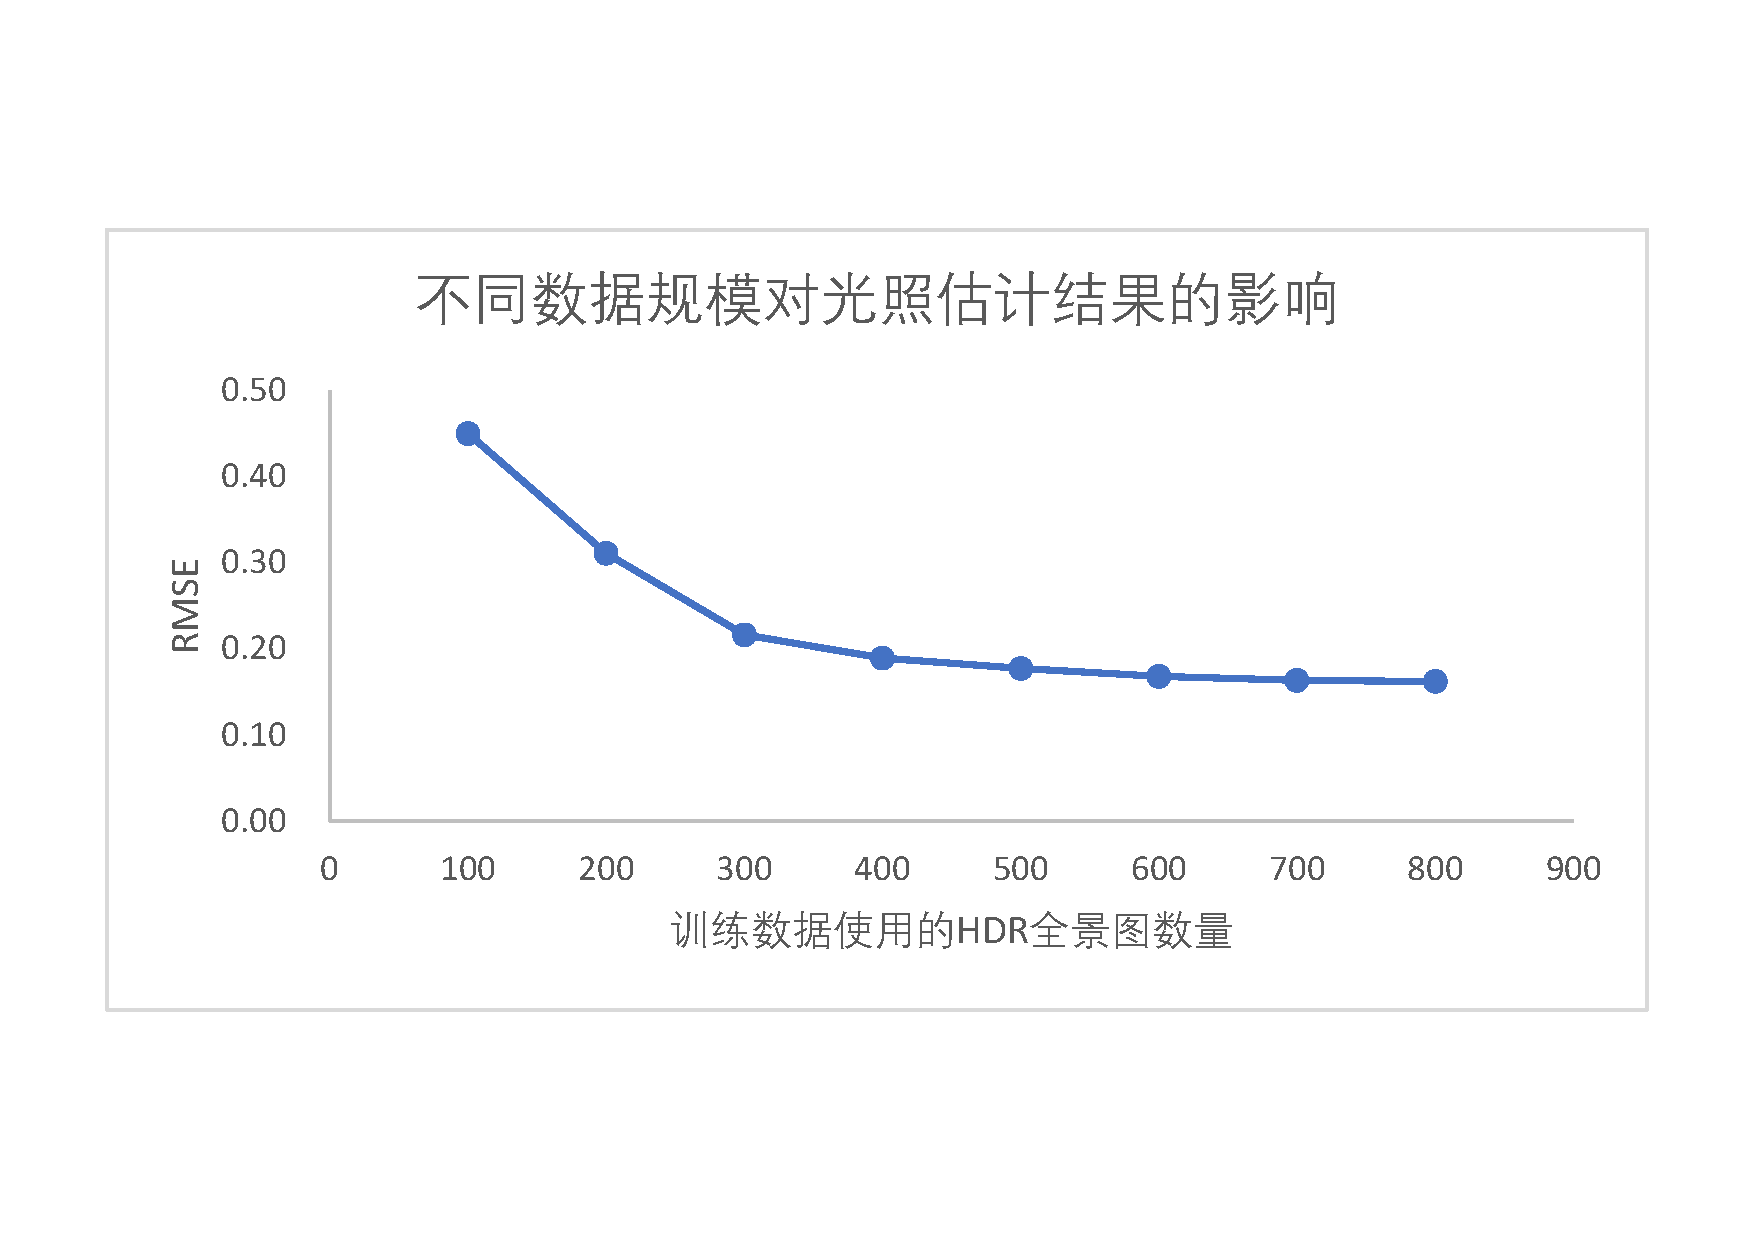
\includegraphics[width=1.0\textwidth]{Img/eval-data-size.pdf}
    \caption[数据规模对光照估计问题影响的趋势图]
    {数据规模对光照估计问题影响的趋势图。可以看出,在数据规模较小时,增加训练数据量能够为光照估计带来巨大的提升,但当数据达到一定的规模时,这种提升达到了饱和,单纯增加训练数据量并不能起到很好的效果,这主要是因为这些场景中包含了一定的重复场景,而在数据中添加更多的重复场景对训练几乎是没有意义的。}
    \label{fig:eval-data-size}
\end{figure}